\documentclass{optica-article}

\journal{opticajournal} % for journals or Optica Open

\articletype{Research Article}

\usepackage{lineno}
\linenumbers % Turn off line numbering for Optica Open preprint submissions.

\begin{document}

\title{Data Recovery and Pulse Position Modulation with a Photon Number Resolving SNSPD}

\author{Author One,\authormark{1} Author Two,\authormark{2,*} and Author Three\authormark{2,3}}

\address{\authormark{1}Peer Review, Publications Department, Optica Publishing Group, 2010 Massachusetts Avenue NW, Washington, DC 20036, USA\\
\authormark{2}Publications Department, Optica Publishing Group, 2010 Massachusetts Avenue NW, Washington, DC 20036, USA\\
\authormark{3}Currently with the Department of Electronic Journals, Optica Publishing Group, 2010 Massachusetts Avenue NW, Washington, DC 20036, USA}

\email{\authormark{*}opex@optica.org} %% email address is required; see note below about the corresponding author designation

% use {asbstract*} to suppress the copyright line. Copyright information will be added in production

\begin{abstract*} 
Photon number resolution is an emerging capability of advanced Superconducting Nanowire Single Photon Detectors. If leveraged to it's full potential, PNR capabilty can have a profound impact on the usefulness of SNSPDs is certain quantum applications including linear optical quantum computing, quantum networks, and quantum sensing. Discrimination of not just the number of photons in an optical pulse but also pulse arrival time with high accuracy is an open problem, complicated by the nuanced way in which these two degrees of freedom are intertwined in the response function of these detectors. In this work we put a differential readout SNSPD to the ultimate test. We test it's capabilities in a Pulse Position Modulation experiment whereby data is sent in the arrival time of optical pulses derived from a 20 GHz optical clock. We show the detector is capable of discriminating the arrival time of photons to 50\textasciitilde ps wide bins with high accuracy while simultaneously providing photon number information about the impinging optical pulses. We find that a careful statistical analysis of the PNR response is necessary to back-out a precise measurement of pulse arrival time.
\end{abstract*}

%%%%%%%%%%%%%%%%%%%%%%%%%%  body  %%%%%%%%%%%%%%%%%%%%%%%%%%
\hypertarget{introduction}{%
\subsection{Introduction}\label{introduction}}

This is the introduction with some latex \(\frac{33}{44}\)

Something unique.

\hypertarget{fig:channel_data}{%
\begin{figure}
\centering
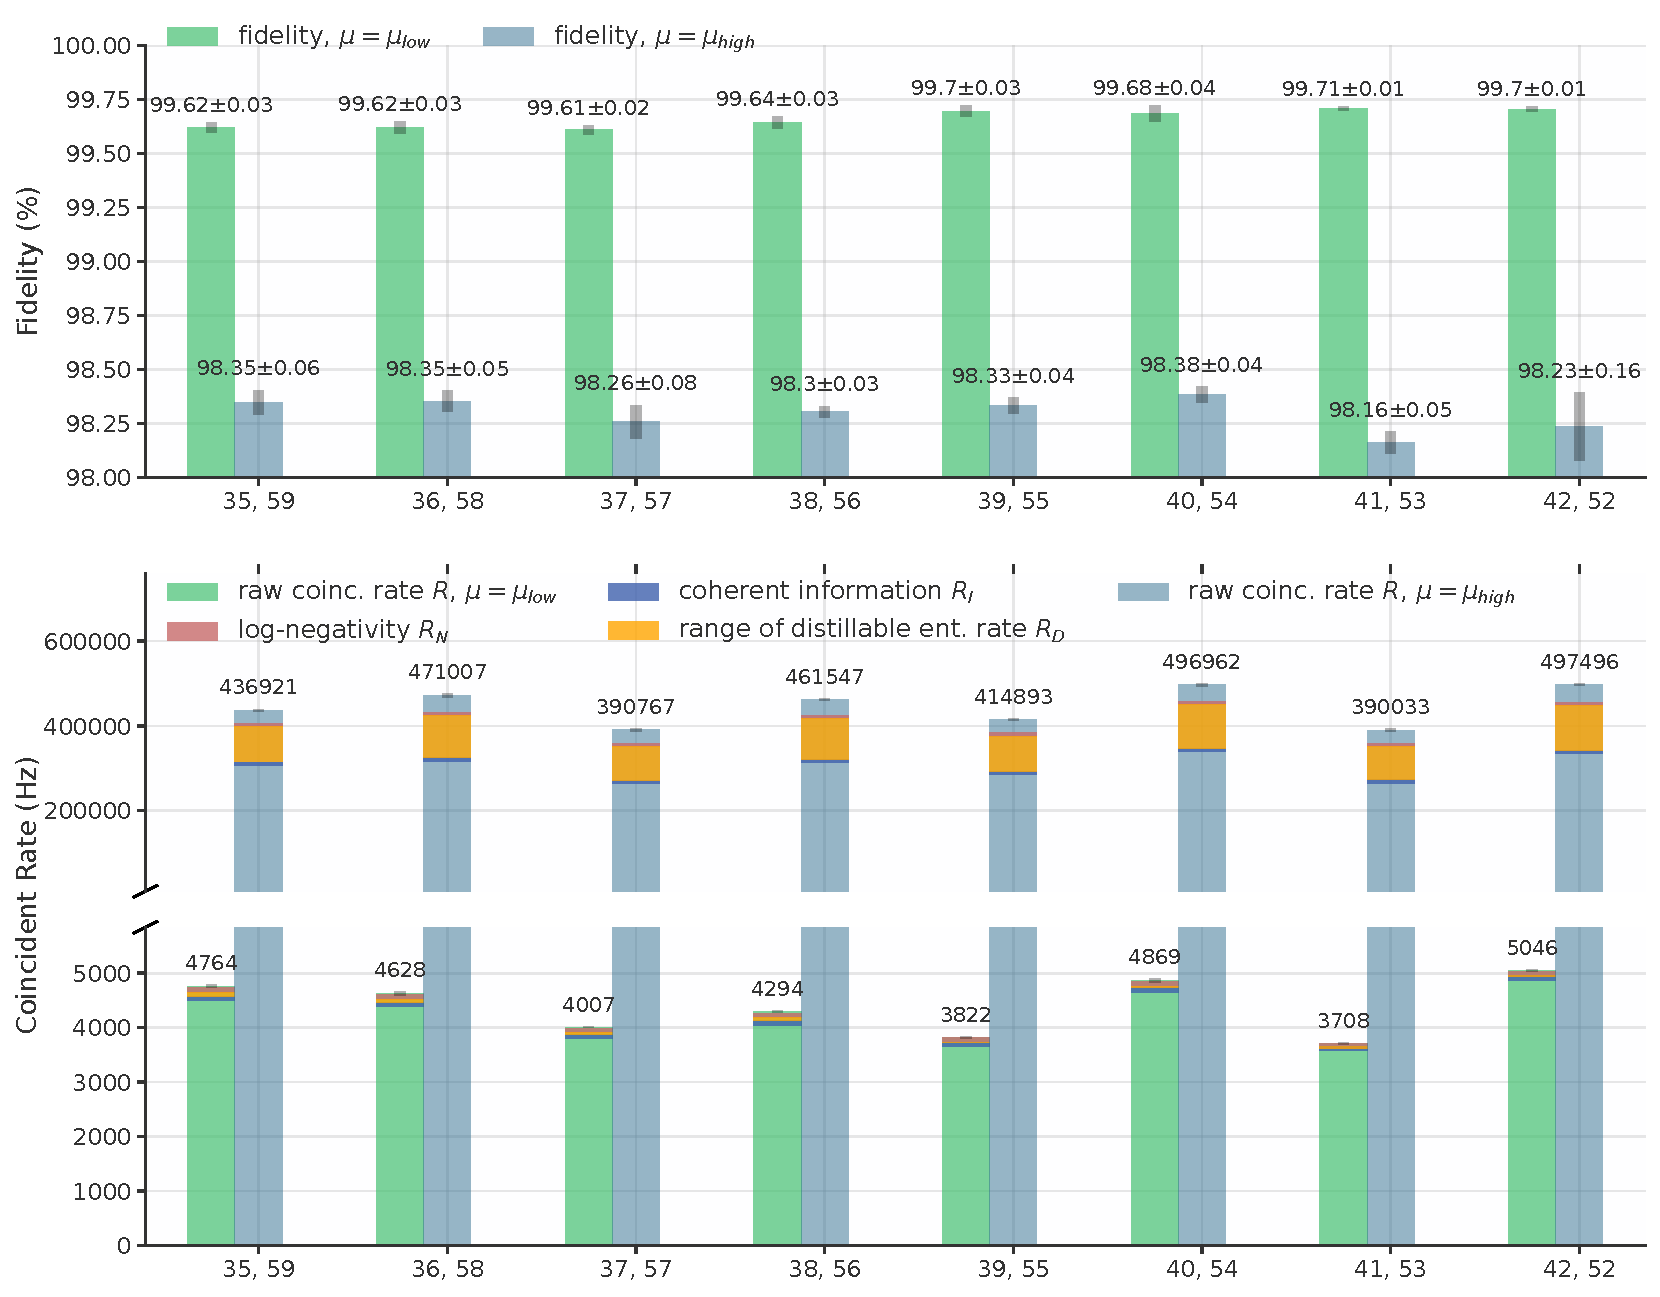
\includegraphics[width=1\textwidth,height=\textheight]{./figs_03/8ch_bar_graph_high_power_light.pdf}
\caption[{Fidelity and rates across 8 channel pairs.}]{\textbf{Fidelity and rates across 8 channel pairs} a) Fidelity for the main 8 channel pairs, measured at a high (5.17 Amps) and a low ( 1.2 Amps) SHG pump power setting. Each power setting results in similar \(\mu\) for all channels: \(\mu_{low}\) = 5.6e-5 \(\pm\) 9e-6 and \(\mu_{high}\) = 6.1e-3 \(\pm\) 3e-4. b) Rate metrics for the 8 channel pairs at the same high and low power settings. The range of possible values for distillable entanglement rate is spanned by the yellow regions, bounded above by log-negativity and below by coherent information. Rates shown assume readout of all 4 available interferometer ports, based on data measured using one port each at Alice and Bob}
\label{fig:channel_data}
\end{figure}
}

\hypertarget{methods}{%
\subsection{Methods}\label{methods}}

This is the methods section with some latex \(\frac{33}{44}\)

Here is citation \cite{Dolinar2011Photon} and here is the rest of the sentence.

\bibliography{references}



\end{document}